\RequirePackage{plautopatch}
\RequirePackage[l2tabu, orthodox]{nag}

\documentclass{jsarticle}
\usepackage{listings,jlisting}
\lstset{
    basicstyle={\ttfamily\small},
    frame=tRBl,
    framesep=10pt,
    breaklines=true,
    linewidth=12cm,
    lineskip=-0.5ex,
    tabsize=2
}
\usepackage[dvipdfmx]{graphicx}
\title{情報科学演習2 C言語課題レポート}

\author{6319050 情報科学科 佐藤駿}
\date{\today}
\begin{document}
\maketitle

\newpage

\section{課題の説明}
郵便番号検索のプログラムを作成せよ.\\
住所から郵便番号を検索する機能と郵便番号から住所を検索する機能を有すること.\\
また,必ずハッシュ(演習でやったチェイン法で良い)を用いること.

\section{アルゴリズムの説明}
プログラムで用いた変数や関数のアルゴリズム・動作について説明する.
\begin{itemize}
    \item \#define n: ハッシュ関数内でmodを取るために使用する数値.
    \item struct cell \*p\_hashtabe[n]: 郵便番号のハッシュテーブル.
    \item struct cell \*a\_hashtabe[n]: 住所のハッシュテーブル.
    \item struct cell: 今回データを保存する構造体.\*p\_codeは郵便番号,\*addressは住所をそれぞれ文字列で保持する.\*p\_next,\*a\_nextはそれぞれ郵便番号と住所のハッシュテーブルで次のデータのポインタを表す.
    \item int hash(char \*key): ハッシュ値を計算する関数.与えられた文字列に対して数値型で各文字の和を取りそれをnで割った余りを返す.
    \item int post\_hash(char \*key): kadai2.cのみに実装. hash関数に掛け算を加えたもの.詳細は考察で説明.
    \item void add(char \*post\_code, char \*address): 受け取った郵便番号と住所をのハッシュ値を計算してハッシュテーブルに登録する.ハッシュ値が衝突した場合はハッシュテーブルの要素の先頭に新しいデータを挿入する.
    \item struct cell *find\_address(char \*address): 住所からハッシュテーブル内の郵便番号を検索する関数.見つからなければNULLを返す.
    \item struct cell *find\_postcode(char \*post\_code): 郵便番号からハッシュテーブル内の住所を検索する関数.見つからなければNULLを返す.
    \item void hash\_info(): ハッシュテーブルの情報を表示する関数.具体的にはハッシュテーブル要素のテーブルサイズの平均と分散を計算して表示を行なう.主に考察で使用.
\end{itemize}
\newpage

\section{プログラムの説明}
kadai.cの主要な関数,main関数の説明を行う.\\
\begin{lstlisting}[caption = kadai.c hash]
int hash(char *key){
    int hashval = 0;
    while(*key!='\0'){
        hashval += *key;
        key++;
    }
    return abs(hashval) % n;
}
\end{lstlisting}
受け取った文字列に含まれる文字コードの和をwhile文で計算し,その絶対値をnで割った余りを返す.ここで絶対値を取っているのは,いくつかの漢字が文字コードの数値型からあふれて負の値をとっている場合があり,modを計算する前に正の値に直すためである.\\

\begin{lstlisting}[caption = kadai.c add]
void add(char *post_code, char *address){
    int p_hash, a_hash;
    p_hash = hash(post_code);
    a_hash = hash(address);
    struct cell *ptr;
    ptr = malloc(sizeof(struct cell));
    ptr->p_code = malloc(sizeof(char)*(strlen(post_code)+1));
    ptr->address = malloc(sizeof(char)*(strlen(address)+1));
    strcpy(ptr->p_code, post_code);
    strcpy(ptr->address, address);
    ptr->p_next = p_hashtable[p_hash];
    p_hashtable[p_hash] = ptr;
    ptr->a_next = a_hashtable[a_hash];
    a_hashtable[a_hash] = ptr;
    return;
}
\end{lstlisting}
まず受け取った郵便番号と住所のハッシュ値を計算する.\\
次に新しいデータを保存するための領域を確保してそこにstrcpyで郵便番号と住所の文字列をそれぞれコピーする.\\
最後に新しいデータの次のポインタをハッシュ値に対応するテーブルの先頭にして,テーブルの先頭をそのデータに更新する.
\newpage

\begin{lstlisting}[caption = kadai.c find\_address find\_post\_code]
struct cell *find_address(char *address){
    struct cell *p;
    int hashval;
    hashval = hash(address);
    p = a_hashtable[hashval];

    while(p!=NULL){
        if(strcmp(address,p->address)==0){
            return p;
        }
        p = p->a_next;
    }
    return NULL;
}

struct cell *find_postcode(char *post_code){
    struct cell *p;
    int hashval;

    hashval = hash(post_code);
    p = p_hashtable[hashval];

    while(p!=NULL){
        if(strcmp(post_code,p->p_code)==0){
            return p;
        }
        p = p->p_next;
    }
    return NULL;
}
\end{lstlisting}
同じ操作なので同時に説明する.\\
まず受け取った文字列のハッシュ値を計算する.\\
次にハッシュ値に対応するテーブルの要素をwhile文で一つずつ調べ,受け取った文字列と同じ要素を見つけたら,その組となっている文字列を返す.\\
対応する要素がなかった場合NULLを返す.\\
\newpage

\begin{lstlisting}[caption = kadai.c hash\_info]
void hash_info(){
    int i, length;
    int p_hashtable_count[n];
    int a_hashtable_count[n];
    int sum=0;
    struct cell *p,*a;

    for(i=0; i< n; i++){
        length = 0;
        p = p_hashtable[i];
        while(p!=NULL){
            length++;
            p = p->p_next;
        }
        // printf("p_hashtable [%d] : %d\n",i,length);
        p_hashtable_count[i] = length;
        sum += length;
    }
    for(i=0; i< n; i++){
        length = 0;
        a = a_hashtable[i];
        while(a!=NULL){
            length++;
            a = a->a_next;
        }
        // printf("a_hashtable [%d] : %d\n",i,length);
        a_hashtable_count[i] = length;
    }
    float average = (float)sum/(float)n;
    float p_variance,a_variance;
    for(i=0; i<n; i++){
        p_variance += (average-p_hashtable_count[i])*(average-p_hashtable_count[i]);
        a_variance += (average-a_hashtable_count[i])*(average-a_hashtable_count[i]);
    }
    p_variance = sqrtf(p_variance);
    a_variance = sqrtf(a_variance);
    printf("Average: %f\n",average);
    p_variance = p_variance/(float)average;
    a_variance = a_variance/(float)average;
    printf("Variance: p_hash %f, a_hash %f\n",p_variance,a_variance);
}
\end{lstlisting}
まずfor文とwhile文でそれぞれのテーブルの要素数がいくつかを数える.その際に全データ数をsumに記録する.\\
次にsumをnで割って各テーブルの平均サイズをaverageに代入する.またfor文で郵便番号と住所のハッシュテーブルサイズの分散を計算して,それぞれp\_variance,a\_varianceに代入する.\\
最後に平均と分散を表示する.\\

\begin{lstlisting}[caption = kadai.c main]
int main(int argc, char *argv[]){
    printf("Hash mod:%d\n",n);
    struct timeval start,end;
    char post_code[256];
    char address[256];
    struct cell *ptr;
    char word[256];

    FILE *fp;
    fp = fopen("postal.txt","r");
    while(fscanf(fp,"%s %s",post_code,address)!=EOF){
        add(post_code, address);
    }
    fclose(fp);

    hash_info();

    if(argc>1){
        fp = fopen(argv[1],"r");
        gettimeofday(&start,NULL);
        while(fscanf(fp,"%s",word)!=EOF){
            // printf("%s\n",word);
            if(word[0]>='0'&&word[0]<='9'){
                ptr = find_postcode(word);
                if(ptr==NULL) continue;
                // printf("->%s\n",ptr->address);
            } else {
                ptr = find_address(word);
                if(ptr==NULL) continue;
                // printf("->%s\n",ptr->p_code);
            }
        }
        gettimeofday(&end,NULL);
        printf("Search time = %lf\n", (end.tv_sec - start.tv_sec) + (end.tv_usec - start.tv_usec)*1.0E-6);
        fclose(fp);
    } else {
        while(scanf("%s", word) != EOF){
            if(word[0]>='0'&&word[0]<='9'){
                ptr = find_postcode(word);
                if(ptr==NULL) continue;
                printf("->%s\n",ptr->address);
            } else if(word[0]=='q') {
                break;
            } else {
                ptr = find_address(word);
                if(ptr==NULL) continue;
                printf("->%s\n",ptr->p_code);
            }
        }
    }
    return 0;
}
\end{lstlisting}
最初にnの値の表示を行う. struct timevalは今回時間計測に使ったtime.hから利用できる構造体である.\\
次にpostal.txtを一行ずつ読み込んでadd関数からデータを追加する.hash\_infoでハッシュテーブルの情報を表示する.\\
最後にメインの検索処理を行う.ここで実行時にコマンドライン引数が与えられているかどうかで異なる動作をするようにしている.\\
まず引数が与えられていた場合その引数と同じ名前の.txtファイルを読み込んで,1行ごとに検索処理を行う.その際に実行にかかった時間を計測して最後に表示を行う.引数が与えられなかった場合は入力待ちの状態となる.与えられた入力に対して,それに対応するデータの文字列を表示する.このとき標準出力は\\
入力文字列\\
→出力文字列\\
となる.与えられた文字列が郵便番号か住所かの判定方法は,先頭の文字が文字コードで'0'から'9'の間であれば郵便番号それ以外なら住所とした.
\newpage

\section{実行結果}
以下にいくつかの実行結果を示す.\\\\\\\\
\begin{figure}[!htbp]
\begin{center}
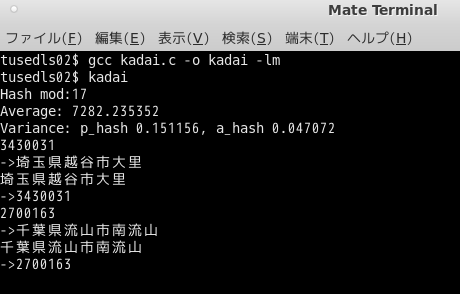
\includegraphics[width=150mm]{1.png}
\caption{kadai.cの実行結果}
\end{center}
コンパイルの際に -lmというオプションを付けているがこれはhash\_infoで使用したmath.hのsqrtfを使うための記述である.\\
郵便番号から住所,住所から郵便番号の検索が正しく行えていることが分かる.
\end{figure}
\newpage

\begin{figure}[!htbp]
\begin{center}
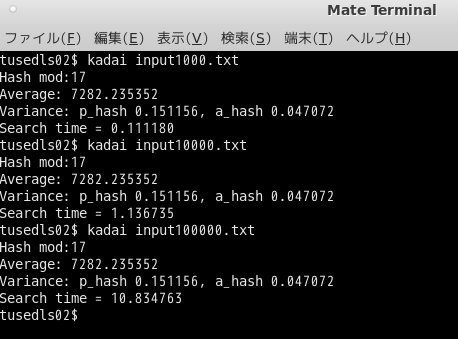
\includegraphics[width=150mm]{2.png}
\caption{kadai.cの実行結果2}
\end{center}
引数として郵便番号と住所が1行ごとに書かれているファイルを渡してそれぞれ処理を行っている.それぞれのファイルには1000,10000,100000行の記述があるのでその数に比例して計測された実行時間が伸びていることが分かる.
\end{figure}
\newpage

\begin{figure}[!htbp]
\begin{center}
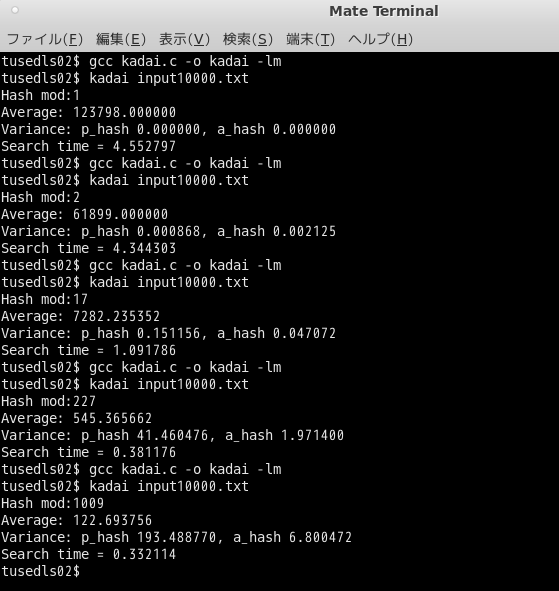
\includegraphics[width=150mm]{3.png}
\caption{kadai.cの実行結果3}
\end{center}
プログラム内のn(hash mod)の数値を変化させて同じ処理を実行させている.hash modの数値を大きくすることで各テーブルの長さを短くできるので同じ処理でも実行時間が大きく変わっていることが確認できる.
\end{figure}
\newpage

\section{考察}
kadai.cの実行結果3を見るとnが大きくなるにつれて郵便番号のハッシュテーブルの長さが住所のものに比べてかなりばらついていることが分かる(分散(Variance)の値より).\\
なぜ郵便番号のハッシュ値が偏っているのかを考える.まず郵便番号は必ず7文字で,さらに文字コードで'0'から'9'の範囲の文字しか使われていない.つまりそれらの和の値は"0000000"(最小値)と"9999999"(最大値)で63しか変わらないことになる.つまり文字コードの和を取ったとしてもnが64以上の場合長さが0のテーブルが発生してしまう.\\
この問題を解決するためには郵便番号のハッシュ値の計算方法を少し改良しなければならない.\\
そこでハッシュ値の計算に次の処理を追加してテーブルの偏りが解消されるか実験を行う.\\\\
・長さ7の数値型配列を用意して郵便番号文字列i桁目に配列のi番目要素を掛けたものの和を計算する.\\\\
今回は$a=[2,3,5,7,11,13,17], b=[2,4,8,16,32,64,128], c=[3,9,27,81,243,729,2187]$の3つの配列を用意して実験を行った.\\
新しいハッシュ関数の実装はkadai2.cに行った.以下に追加したpost\_hash関数を示す.\\
\begin{lstlisting}[caption = kadai2.c post\_hash]
int post_hash(char *key){
    int hashval = 0;
    int a[] = {2,3,5,7,11,13,17};
    int b[] = {2,4,8,16,32,64,128};
    int c[] = {3,9,27,81,243,729,2187};
    int i;
    for(i=0;i<7;i++){
        hashval += c[i] * (*key);
        key++;
    }
    return abs(hashval) % n;
}
\end{lstlisting}
このプログラム中では配列cの要素が各文字にかけられていることになる.\\
\newpage
以下に実行結果を示す.\\
\begin{figure}[!htbp]
\begin{center}
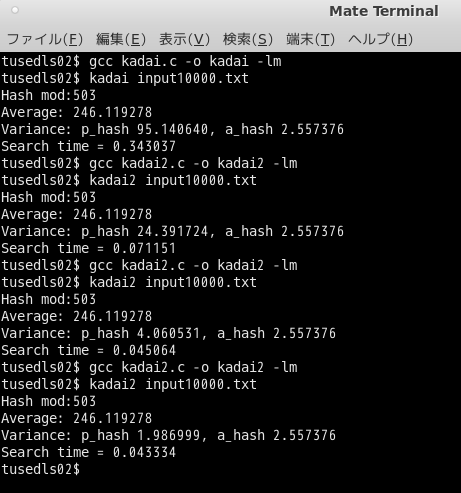
\includegraphics[width=150mm]{4.png}
\caption{kadai.c kadai2.cの実行結果の比較}
\end{center}
kadai2.cは3回実行されているが,上から順にa,b,cの配列をそれぞれ使った場合の実行結果となっている.kadai.cに比べてkadai2.cの方が郵便番号のハッシュテーブルの偏りが解消され明らかに実行時間が短くなっていることが確認できる.さらにkadai2.c内でもa,b,cの順に偏りが小さく実行時間が短くなっている.これは掛けられる値にある程度大きさの幅がある方が,より多様な値を取れることを示している.\\
よってハッシュ関数を工夫することで計算量を増やさなくてもハッシュテーブルの偏りを解消できることが分かった.
\end{figure}
\end{document}
